\documentclass[aspectratio=169,11pt]{beamer}
\usetheme{Madrid}
\usecolortheme{default}
\setbeamertemplate{navigation symbols}{}
\setbeamertemplate{caption}{\insertcaption}
\setbeamerfont{block title}{size=\small}
\setbeamerfont{frametitle}{size=\large}

\usepackage[T1]{fontenc}
\usepackage[utf8]{inputenc}
\usepackage{graphicx}
\usepackage{booktabs}
\usepackage{amsmath}
\usepackage{tikz}
\usetikzlibrary{positioning, arrows.meta, shapes.geometric, backgrounds, fit, calc}

\definecolor{jsyred}{HTML}{8B1A1A}
\definecolor{jsyamber}{HTML}{D98B2B}
\definecolor{jsyblue}{HTML}{2C4A6B}
\definecolor{jsygreen}{HTML}{2E6B3E}
\newcommand{\kn}[1]{{\color{jsyred}\bfseries #1}}

% ---- Slido poll styling ----
% a poll banner at the top of a poll slide
\newcommand{\pollbanner}[1]{%
  \begin{center}\colorbox{jsyblue}{\makebox[0.96\linewidth][l]{\textcolor{white}{\footnotesize\hspace{0.3em}\textbf{Slido poll} \textbullet\ #1\hspace{0.3em}}}}\end{center}}
% one option row
\newcommand{\opt}[2]{\makebox[1.1em][l]{\textbf{#1}} #2\par\vspace{0.35em}}

\title[JSY and financial incentives]{Financial Incentives and Facility Births:\\Evidence from India's Janani Suraksha Yojana}
\subtitle{{\small Powell-Jackson, Mazumdar \& Mills (2015), \emph{Journal of Health Economics} 43, 154--169}}
\author[Your Name]{Your Name}
\institute[Ashoka University]{Health Economics}
\date{November 2026}

\begin{document}

% ===============================================================
\begin{frame}\titlepage\end{frame}

% ===============================================================
\begin{frame}{Outline}
  \tableofcontents
\end{frame}

% ===============================================================
\section{Introduction}
% ===============================================================
\begin{frame}{\phantom{Poll}}
  \pollbanner{let us start with a poll}
  \vspace{0.6em}
  \begin{center}\large\textbf{In the policies we have studied, does expanding\\\emph{access} to a health input usually deliver the\\\emph{health outcome} it was meant to?}\end{center}
  \vspace{0.9em}
  \begin{columns}\column{0.12\textwidth}\column{0.76\textwidth}
    \opt{A}{Usually yes --- getting people to use a service is the hard part}
    \opt{B}{Only if the \emph{quality} of the service is also good}
    \opt{C}{Only if people actually \emph{use} what they are given, not just own it}
    \opt{D}{Rarely --- behaviour and incentives usually undo the gains}
  \column{0.12\textwidth}\end{columns}
  \vspace{0.5em}
  \begin{center}\footnotesize Hold that thought. We test it today with one large programme.\end{center}
\end{frame}

% ===============================================================
\begin{frame}{Motivation: a recurring theme in this course}
  \begin{columns}[T]
    \column{0.54\textwidth}
    A theme runs through the course: a policy can \textbf{expand access} to a health input, yet the \textbf{health outcome does not follow}.
    \vspace{0.5em}

    Our Week 9 paper on \textbf{Ujjwala (LPG)}, Gupta et al. (2019), is one case. LPG ownership rose to about three-quarters of rural households, but about three-quarters of them \textbf{still burned solid fuel}. Ownership did not become clean-air use.
    \vspace{0.5em}

    This paper asks the same kind of question for a \textbf{cash incentive} to give birth in a facility.
    \column{0.44\textwidth}
    \begin{block}{The pattern to test}
      \centering
      \vspace{0.2em}
      subsidy / incentive\\
      $\downarrow$\\
      \textbf{more of the input}\\
      {\footnotesize (facility births, LPG)}\\
      $\downarrow$ \textcolor{jsyred}{\textbf{?}}\\
      \textbf{better health outcome}\\
      {\footnotesize (survival, clean air)}
      \vspace{0.2em}
    \end{block}
    {\footnotesize The question mark is where this paper does its work.}
  \end{columns}
\end{frame}

% ===============================================================
\begin{frame}{\phantom{Poll}}
  \pollbanner{respond on Slido}
  \vspace{0.5em}
  \begin{center}\large\textbf{An earlier \emph{Lancet} study found large gains from the JSY.\\What do you think this paper finds for newborn mortality?}\end{center}
  \vspace{0.8em}
  \begin{columns}\column{0.1\textwidth}\column{0.8\textwidth}
    \opt{A}{A large fall in deaths, matching the earlier study}
    \opt{B}{A small but clear fall}
    \opt{C}{No statistically detectable effect}
    \opt{D}{Deaths actually rose}
  \column{0.1\textwidth}\end{columns}
  \vspace{0.4em}
  \begin{center}\footnotesize The next slide is the answer.\end{center}
\end{frame}

% ===============================================================
\begin{frame}{The question}
  \begin{columns}[T]
    \column{0.58\textwidth}
    The Janani Suraksha Yojana (JSY) pays women to give birth in a public facility. The expected result is clear. More women use skilled care, so fewer newborns die.
    \vspace{0.5em}

    An earlier \emph{Lancet} study supported this. It found facility births up \kn{40+ pp} and neonatal deaths down \kn{2--6 per 1000}.
    \vspace{0.5em}

    This paper does not find that result. The design is tighter and the data are larger. The effect on mortality is \kn{not different from zero}. The cash also changes behaviours that the policy did not target.
    \column{0.40\textwidth}
    \begin{block}{Three questions}
      \begin{enumerate}
        \item Did the cash raise \textbf{use} of care?
        \item Did use lower \textbf{mortality}?
        \item What \textbf{else} did it change?
      \end{enumerate}
    \end{block}
    \begin{alertblock}{Why it is difficult}
      There is no randomisation. The programme started where need was large. So a simple comparison is confounded.
    \end{alertblock}
  \end{columns}
\end{frame}

% ===============================================================
\begin{frame}{Context: high mortality, already in decline}
  \begin{columns}[T]
    \column{0.52\textwidth}
    \begin{itemize}
      \item India had approximately \kn{72{,}000} maternal deaths per year --- the largest number of any country
      \item Maternal mortality fell \kn{47\%} (398 to 178 per 100{,}000) from 1997--98 to 2010--12
      \item State differences are large: Kerala is approximately 5 times lower than the poorest northern states
    \end{itemize}
    \vspace{0.3em}
    \begin{alertblock}{The identification problem}
      Outcomes improved in all states. The design must separate the JSY effect from this national trend.
    \end{alertblock}
    \column{0.46\textwidth}
    \begin{block}{Raw means, before and during the JSY (Table 1)}
      \centering\footnotesize
      \begin{tabular}{lcc}
        \toprule & Before & During \\ \midrule
        Neonatal mortality /1000 & 33.0 & \kn{26.6} \\
        Facility births (\%) & 38.7 & \kn{43.7} \\
        \quad public & 20.0 & 25.5 \\
        \quad private & 18.7 & 18.2 \\
        Breastfeeding $<$1h (\%) & 31.1 & \kn{39.9} \\
        \bottomrule
      \end{tabular}
    \end{block}
    \footnotesize The means move in the expected direction. But a correlation is not the causal effect of the JSY.
  \end{columns}
\end{frame}

% ===============================================================
\section{Background (\S2)}
% ===============================================================
\begin{frame}{The programme: a conditional cash transfer (\S2.1)}
  \begin{columns}[T]
    \column{0.54\textwidth}
    \begin{itemize}
      \item The programme started in 2005 under the National Rural Health Mission
      \item It pays cash to a woman who gives birth in a \textbf{public} facility (or an accredited private one), within one week
      \item Community health workers (ASHAs) get \kn{Rs 200--600} for each delivery they bring in --- a supply-side payment
      \item The payment is \textbf{larger in low-performing states}
    \end{itemize}
    \vspace{0.2em}
    \footnotesize Scale (2007/08): \kn{Rs 8.8 bn} ($\approx$\$207m) per year, \kn{7.1m} beneficiaries. A public delivery costs approximately \$25.
    \column{0.44\textwidth}
    \begin{center}
    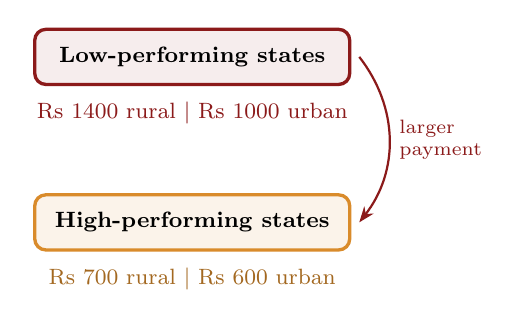
\begin{tikzpicture}[font=\footnotesize]
      \node[draw=jsyred, very thick, fill=jsyred!8, rounded corners, minimum width=4cm, minimum height=0.7cm, align=center] (lp) {\textbf{Low-performing states}};
      \node[below=0.08cm of lp, text=jsyred] (lpv) {Rs 1400 rural \textbar{} Rs 1000 urban};
      \node[draw=jsyamber, very thick, fill=jsyamber!10, rounded corners, below=0.75cm of lpv, minimum width=4cm, minimum height=0.7cm, align=center] (hp) {\textbf{High-performing states}};
      \node[below=0.08cm of hp, text=jsyamber!75!black] {Rs 700 rural \textbar{} Rs 600 urban};
      \draw[-{Stealth[length=2mm]}, thick, jsyred] ($(lp.east)+(0.1,0)$) to[bend left=38] node[right,font=\scriptsize,align=left]{larger\\payment} ($(hp.east)+(0.1,0)$);
    \end{tikzpicture}
    \end{center}
    {\footnotesize\centering This asymmetry is important. It returns in the heterogeneity results.}
  \end{columns}
\end{frame}

% ===============================================================
\begin{frame}{Anticipated effects (\S2.2): the causal chain}
  \vspace{0.2em}
  \begin{center}
  \resizebox{0.98\textwidth}{!}{%
  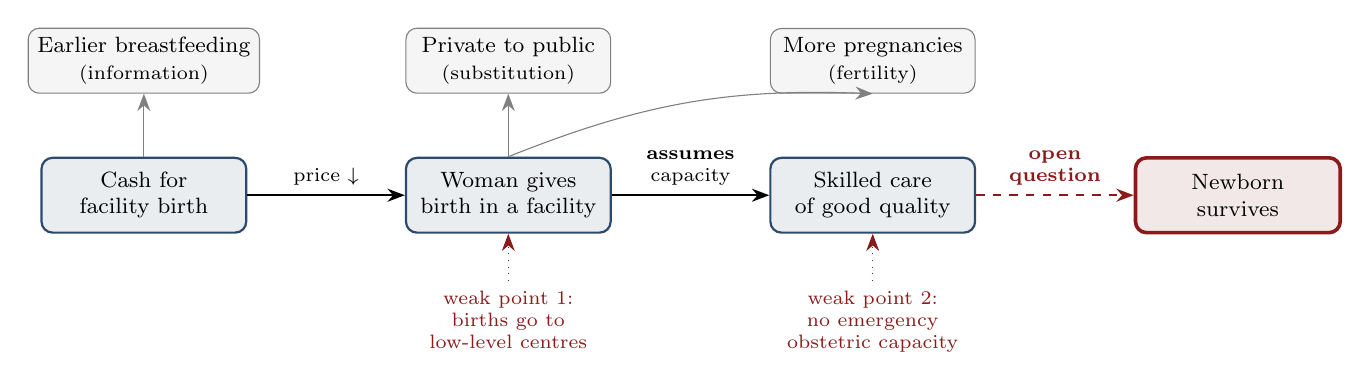
\begin{tikzpicture}[font=\footnotesize, >={Stealth[length=2.2mm]},
      stage/.style={draw, rounded corners, minimum height=0.95cm, minimum width=2.6cm, align=center, fill=jsyblue!10, draw=jsyblue, line width=0.8pt},
      target/.style={fill=jsyred!10, draw=jsyred, line width=1.3pt},
      side/.style={draw, rounded corners, minimum height=0.8cm, minimum width=2.6cm, align=center, fill=gray!8, draw=gray},
      lbl/.style={font=\scriptsize, align=center}]
    \node[stage] (cash) {Cash for\\facility birth};
    \node[stage, right=2.0cm of cash] (use) {Woman gives\\birth in a facility};
    \node[stage, right=2.0cm of use] (care) {Skilled care\\of good quality};
    \node[stage, target, right=2.0cm of care] (surv) {Newborn\\survives};
    \draw[->, thick] (cash) -- node[lbl, above]{price $\downarrow$} (use);
    \draw[->, thick] (use) -- node[lbl, above]{\textbf{assumes}\\capacity} (care);
    \draw[->, thick, dashed, jsyred] (care) -- node[lbl, above, text=jsyred]{\textbf{open}\\\textbf{question}} (surv);
    \node[lbl, below=0.6cm of use, text=jsyred] (b1) {weak point 1:\\births go to\\low-level centres};
    \node[lbl, below=0.6cm of care, text=jsyred] (b2) {weak point 2:\\no emergency\\obstetric capacity};
    \draw[jsyred, ->, dotted] (b1) -- (use);
    \draw[jsyred, ->, dotted] (b2) -- (care);
    \node[side, above=0.8cm of use] (subst) {Private to public\\\scriptsize(substitution)};
    \node[side, above=0.8cm of care] (preg) {More pregnancies\\\scriptsize(fertility)};
    \node[side, above=0.8cm of cash] (bf) {Earlier breastfeeding\\\scriptsize(information)};
    \draw[->, gray] (cash.north) -- (bf.south);
    \draw[->, gray] (use.north) -- (subst.south);
    \draw[->, gray] (use.north) to[bend left=12] (preg.south);
  \end{tikzpicture}}
  \end{center}
  \vspace{0.2em}
  \begin{center}{\small The cash pays for stage 1. Newborns survive only if stages 2 and 3 also hold.}\end{center}
\end{frame}

% ===============================================================
\begin{frame}{Anticipated effects (\S2.2): what theory predicts}
  The authors set out the predictions before they look at the data. Standard theory gives one main effect and three side effects.
  \vspace{0.3em}
  \begin{columns}[T]
    \column{0.5\textwidth}
    \begin{block}{Main effect: more use}
      {\footnotesize A short-term price cut raises demand for facility care. But the effect on health is uncertain. It depends on the quality of care in the facility, which may be low.}
    \end{block}
    \begin{block}{Substitution}
      {\footnotesize The cash is for public facilities only. So some women move from private to public care. This is a transfer between providers, not a net rise in facility use.}
    \end{block}
    \column{0.5\textwidth}
    \begin{block}{Fertility}
      {\footnotesize Payment per birth is an implicit reward for a birth. It can raise fertility --- a shorter interval between births, or more children over a lifetime.}
    \end{block}
    \begin{block}{Information}
      {\footnotesize More contact with staff can change behaviour at birth, for example earlier breastfeeding or antiseptic cord care.}
    \end{block}
  \end{columns}
  \vspace{0.2em}
  \footnotesize The study tests all four. The side effects are the paper's contribution: earlier work looked at use and mortality only.
\end{frame}

% ===============================================================
\begin{frame}{Evidence on the JSY (\S2.3): the result this paper revisits}
  \begin{columns}[T]
    \column{0.52\textwidth}
    \textbf{Lim et al. (2010), \emph{Lancet}} is the main prior study. It used three identification strategies:
    \begin{enumerate}
      \item \textbf{Individual-level matching}
      \item \textbf{Before-and-after} comparison
      \item \textbf{District-level difference-in-differences}
    \end{enumerate}
    \vspace{0.2em}
    {\footnotesize The headline results came from strategies 1 and 2. The difference-in-differences result (strategy 3) was weaker and got less emphasis.}
    \column{0.46\textwidth}
    \begin{alertblock}{Why this paper doubts strategy 1 and 2}
      {\footnotesize
      \begin{itemize}
        \item Matching has low power and \textbf{reverse selection}: women who give birth in a facility are not a random group
        \item Before-and-after relies on a strong assumption of \textbf{no other change} over the period
      \end{itemize}}
    \end{alertblock}
    {\footnotesize This paper uses the stronger design (strategy 3) and finds the mortality effect does not hold.}
  \end{columns}
\end{frame}

% ===============================================================
\section{Data (\S3)}
% ===============================================================
\begin{frame}{Data: the District Level Health Survey (\S3.1)}
  \begin{columns}[T]
    \column{0.5\textwidth}
    \begin{block}{Two cross-sections}
      \begin{itemize}
        \item DLHS-2 (2002--04): 507{,}622 women, 593 districts
        \item DLHS-3 (2007--08): 643{,}944 women, 611 districts
        \item \kn{587} districts are in both rounds and form the sample
        \item Births 2001--2008 (financial years)
      \end{itemize}
    \end{block}
    \column{0.5\textwidth}
    \begin{block}{Measures}
      \begin{itemize}
        \item \textbf{Outcomes} from the birth histories: facility use, neonatal and one-day mortality
        \item \textbf{JSY coverage}: the share of public-facility mothers who got the cash, by district and year
        \item \textbf{Unintended outcomes}: pregnancy and breastfeeding (DLHS-3)
      \end{itemize}
    \end{block}
  \end{columns}
  \vspace{0.3em}
  \footnotesize Each observation is a woman's most recent delivery (use equations) or a live birth (mortality equations). For pregnancy, the unit is a woman-year, from DLHS-3 only.
\end{frame}

% ===============================================================
\begin{frame}{The coverage measure, and its weakness (\S3.2)}
  \begin{columns}[T]
    \column{0.54\textwidth}
    \textbf{Definition.} $\mathrm{JSY}_{dt}$ is the number of women who got the cash, as a share of women who gave birth in a public facility in district $d$, year $t$.
    \vspace{0.4em}

    \textbf{Why a share, not a count.} It measures how far the programme reached, by district and year. The authors argue this is a \textbf{supply-side} measure, set by administration, not by demand.
    \column{0.44\textwidth}
    \begin{alertblock}{The built-in problem}
      {\footnotesize The cash goes to women who give birth in a facility. So coverage is \textbf{mechanically linked} to the facility-birth rate: the outcome is in the denominator of the treatment.}
    \end{alertblock}
    {\footnotesize This is why the paper leans on district fixed effects and cross-district variation, not on the level of coverage itself.}
  \end{columns}
\end{frame}

% ===============================================================
\section{Empirical strategy (\S4)}
% ===============================================================
\begin{frame}{The variation: staggered district roll-out}
  \begin{center}
    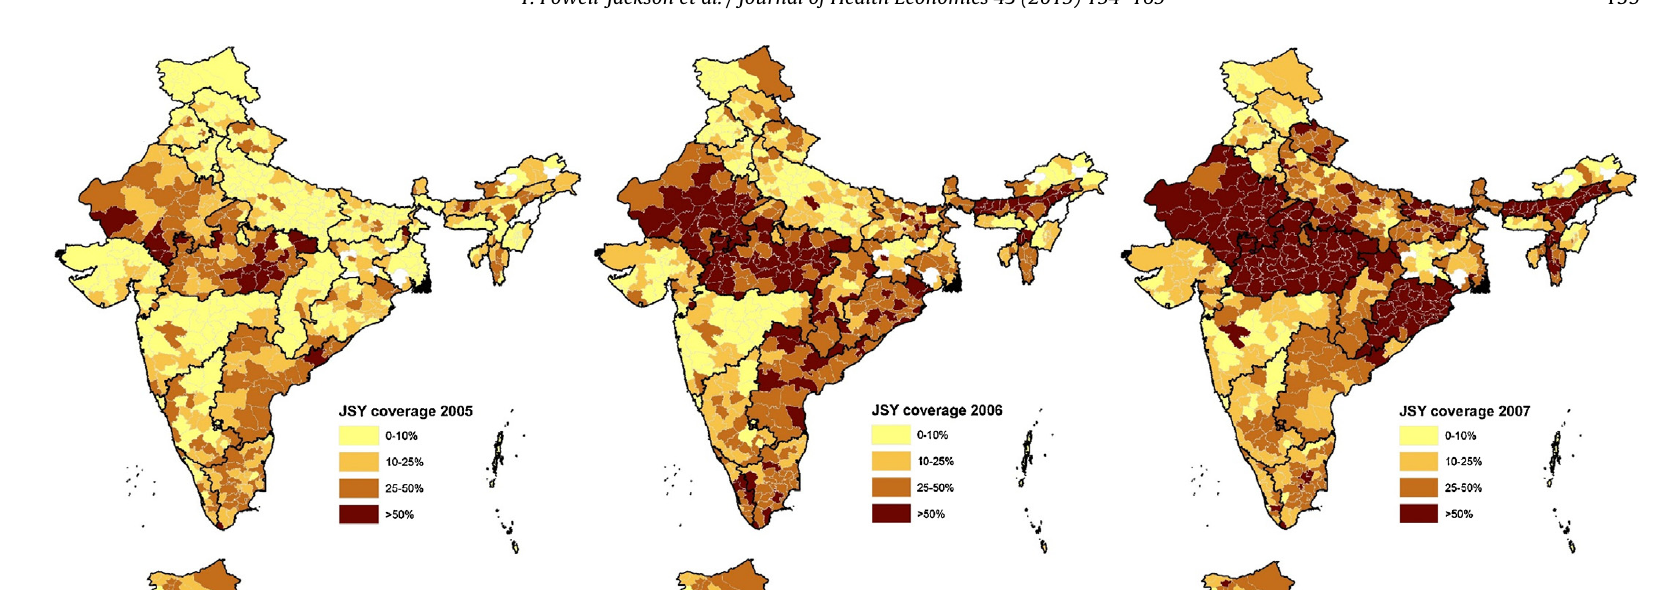
\includegraphics[width=0.88\textwidth]{crop_fig1_top.png}
  \end{center}
  \vspace{-0.1em}
  \begin{columns}[T]
    \column{0.62\textwidth}
    {\footnotesize From 2005 to 2007 the map gets darker as coverage rises. This timing identifies the effect, after district and year fixed effects.}
    \column{0.36\textwidth}
    \begin{alertblock}{\footnotesize The threat}
      {\footnotesize The dark districts are in the poor northern belt. Adoption is \textbf{not random}. It follows need.}
    \end{alertblock}
  \end{columns}
  {\scriptsize Figure 1 (top row), Powell-Jackson et al. (2015). Darker = higher coverage.}
\end{frame}

% ===============================================================
\begin{frame}{The strategy: difference-in-differences}
  The authors compare the change in outcomes across districts with different growth in JSY coverage. The method has three steps.
  \vspace{0.3em}
  \begin{enumerate}
    \item A district fixed effect removes everything about a district that does not change over time (its wealth, its geography, its base level of care)
    \item A year fixed effect removes any shock common to all districts in a year (the national decline in mortality)
    \item What remains is the link between the \emph{rise} in a district's coverage and the \emph{change} in its outcomes
  \end{enumerate}
  \vspace{0.3em}
  \begin{alertblock}{The identifying assumption}
    {\footnotesize Without the JSY, high-coverage and low-coverage districts would have followed \textbf{parallel trends}. You cannot test this directly. The paper probes it with pre-trends (\S5.4).}
  \end{alertblock}
\end{frame}

% ===============================================================
\begin{frame}{The specification, term by term (Eq. 1)}
  \[
    y_{idt} = \beta_0 + \beta_1\,\mathrm{JSY}_{dt} + \vartheta_t Z_d\beta_2 + X_{idt}\beta_3 + \omega_d + \tau_t + \varepsilon_{idt}
  \]
  \vspace{0.2em}
  {\footnotesize\begin{tabular}{@{}p{2.2cm}p{11.5cm}@{}}
    \toprule
    $y_{idt}$ & Outcome for woman $i$, district $d$, year $t$: facility use, or neonatal/one-day mortality \\
    $\mathrm{JSY}_{dt}$ & Coverage, as \textbf{three dummies}: 10--25\%, 25--50\%, $>$50\% (reference: $<$10\%). $\beta_1$ is the effect at each level \\
    $Z_d$ & Three district traits: below-poverty-line share, tribal share, mean wealth asset score \\
    $\vartheta_t Z_d$ & Those traits \textbf{interacted with year} --- lets poor and tribal districts follow their own trends \\
    $X_{idt}$ & Household controls: mother's and husband's education, maternal age, wealth, recall period, and dummies for residence, religion, ethnicity, parity, multiple birth, survey round \\
    $\omega_d,\ \tau_t$ & District and year \textbf{fixed effects} \\
    $\varepsilon_{idt}$ & Error, \textbf{clustered by district} \\
    \bottomrule
  \end{tabular}}
\end{frame}

% ===============================================================
\section{Main results (\S5)}
% ===============================================================
\begin{frame}{\phantom{Poll}}
  \pollbanner{respond on Slido}
  \vspace{0.5em}
  \begin{center}\large\textbf{The cash reached districts at different intensities.\\Where do you expect the effect on facility births?}\end{center}
  \vspace{0.8em}
  \begin{columns}\column{0.1\textwidth}\column{0.8\textwidth}
    \opt{A}{It rises smoothly with coverage, at every level}
    \opt{B}{Only in districts with the highest ($>$50\%) coverage}
    \opt{C}{Strongest at low coverage, then it flattens}
    \opt{D}{No effect at any level}
  \column{0.1\textwidth}\end{columns}
\end{frame}

% ===============================================================
\begin{frame}{Use of care (\S5.1, Table 3)}
  \vspace{-0.2em}
  \begin{center}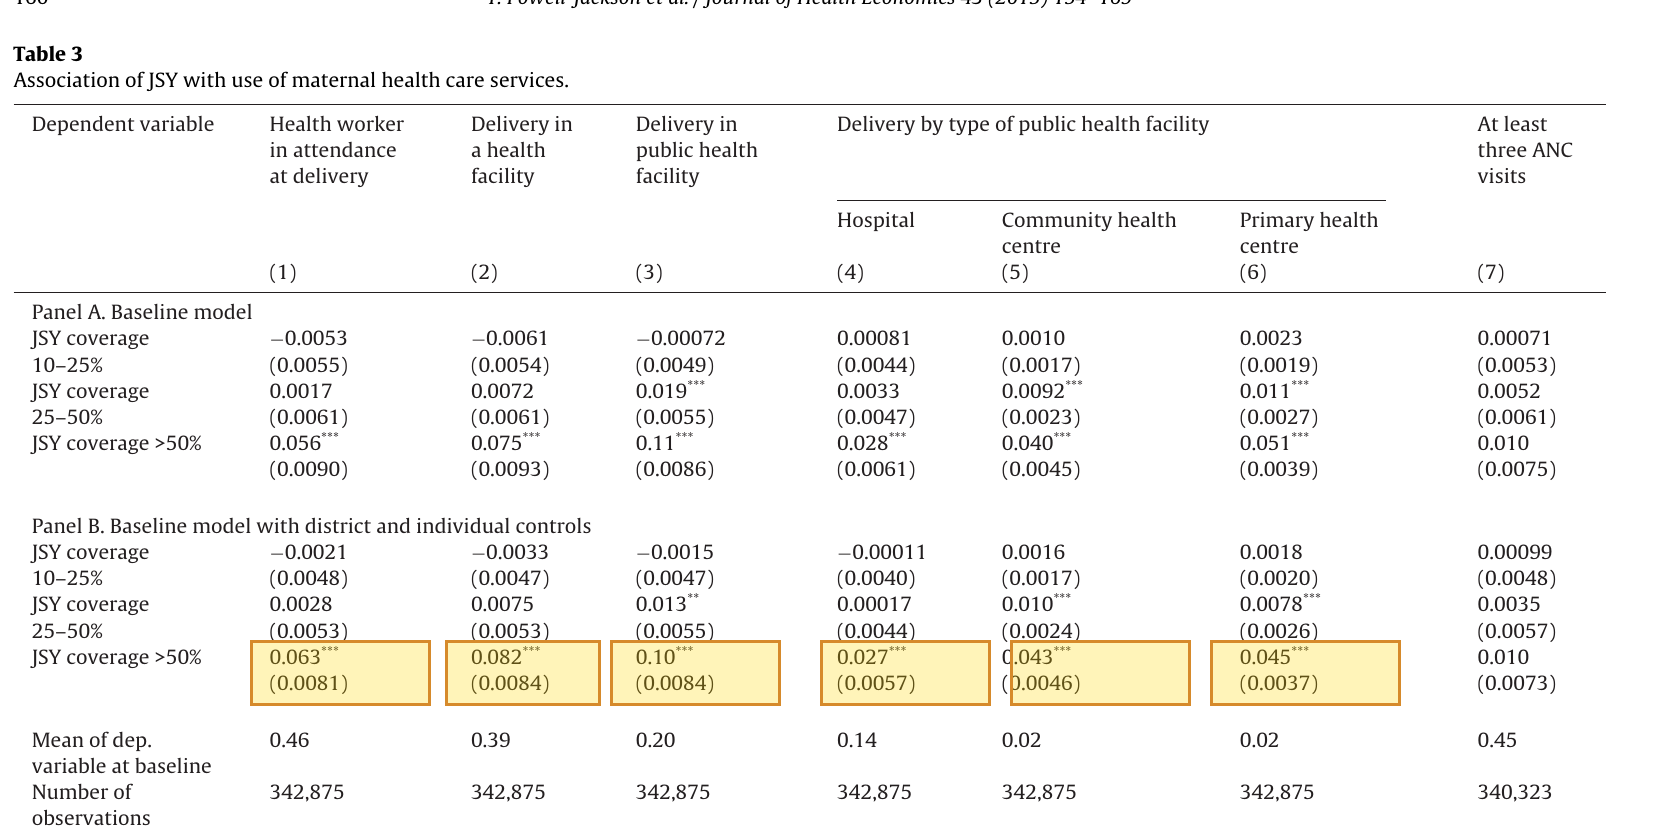
\includegraphics[width=0.80\textwidth]{crop_t3_hl.png}\end{center}
  \begin{columns}[T]
    \column{0.5\textwidth}
    {\footnotesize \colorbox{jsyamber!30}{Boxed} = the significant $>$50\% coefficients with full controls (Panel B). The effect appears \textbf{only at $>$50\%} coverage: facility births \kn{+8 pp}, public births \kn{+10 pp}.}
    \column{0.5\textwidth}
    {\footnotesize The rise is in \textbf{community and primary centres} (cols 5--6), not hospitals. ANC (col 7) is flat and unboxed --- a falsification check.}
  \end{columns}
\end{frame}

% ===============================================================
\begin{frame}{Mortality (\S5.1, Table 4)}
  \begin{columns}[c]
    \column{0.56\textwidth}
    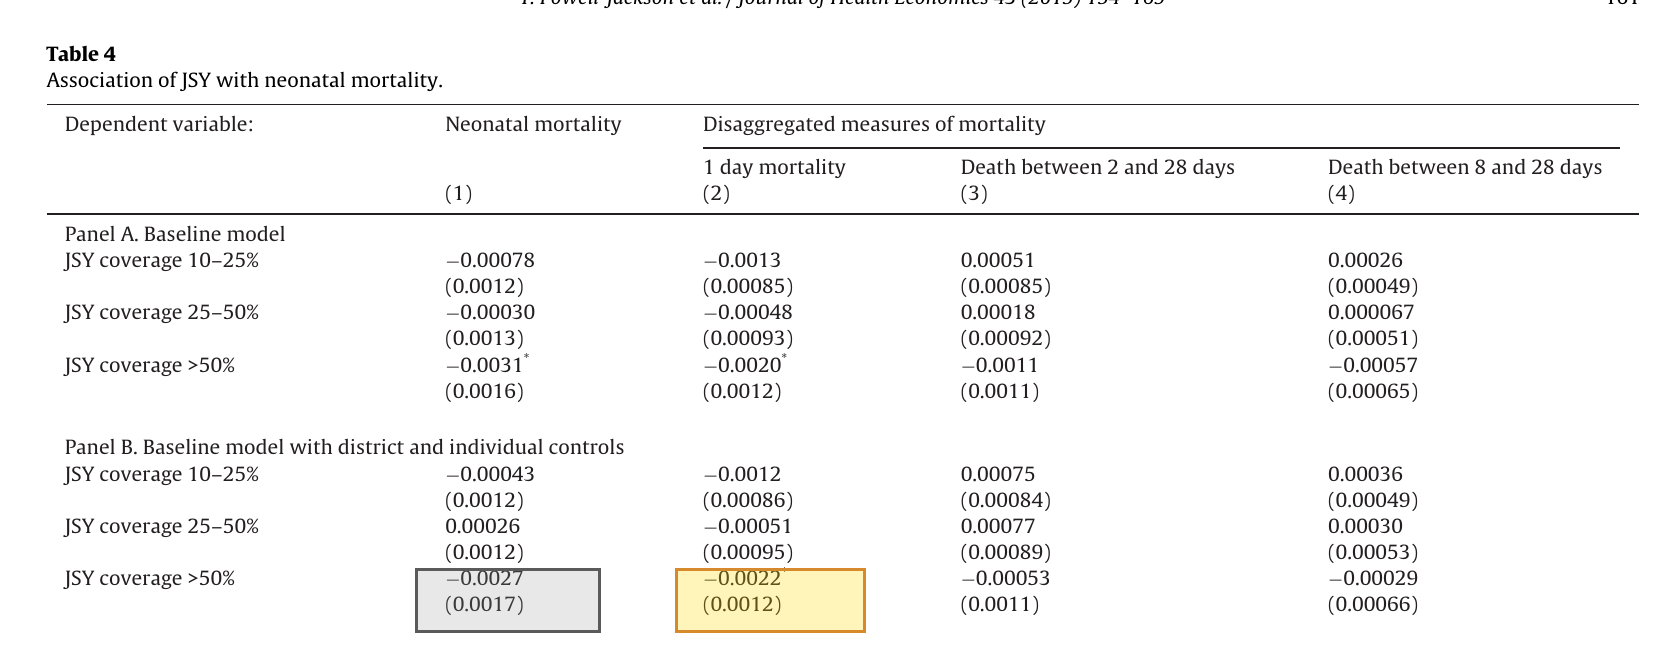
\includegraphics[width=\textwidth]{crop_t4_hl.png}
    \column{0.42\textwidth}
    \begin{itemize}
      \item \colorbox{gray!25}{Grey} = the headline result: neonatal mortality \kn{$-2.7$/1000}, \textbf{not significant} (base 31)
      \item \colorbox{jsyamber!30}{Amber} = one-day deaths $-2.2$, significant at the \textbf{10\% level only}
      \item With full controls, the 95\% CI rules out a fall larger than 5.9/1000 --- the size \emph{Lim et al.} reported
    \end{itemize}
  \end{columns}
  \vspace{0.1em}
  \begin{center}{\small The correct reading is ``no measurable effect'', not ``no effect''.}\end{center}
\end{frame}

% ===============================================================
\begin{frame}{\phantom{Poll}}
  \pollbanner{respond on Slido}
  \vspace{0.5em}
  \begin{center}\large\textbf{Facility births rose, but newborn deaths did not fall.\\Why, according to the authors?}\end{center}
  \vspace{0.8em}
  \begin{columns}\column{0.1\textwidth}\column{0.8\textwidth}
    \opt{A}{The extra births went to low-level centres that cannot handle complications}
    \opt{B}{The rise in facility use was simply too small to move mortality}
    \opt{C}{Many "new" facility births were just women switching from private care}
    \opt{D}{The women drawn in were low-risk, so there were few deaths to prevent}
  \column{0.1\textwidth}\end{columns}
\end{frame}

% ===============================================================
\begin{frame}{The authors' explanation for the mortality result}
  \begin{columns}[T]
    \column{0.56\textwidth}
    The authors call this \emph{``a persuasive explanation''}:
    \begin{enumerate}
      \item The rise in use was modest (8 pp on a 39\% base)
      \item The programme sent women \textbf{predominantly to facilities below the district hospital} --- primary and community centres (Table 3, cols 5--6)
      \item The purpose of those facilities \emph{``was not to manage life-threatening complications''}
    \end{enumerate}
    \column{0.42\textwidth}
    \begin{block}{In the authors' words (\S5.1)}
      {\footnotesize ``However good the quality of care in health institutions below the district hospital, it may remain inadequate to save the lives of women and [newborns].''}
    \end{block}
  \end{columns}
\end{frame}

% ===============================================================
\begin{frame}{Cost-effectiveness (\S5.2)}
  \begin{center}
  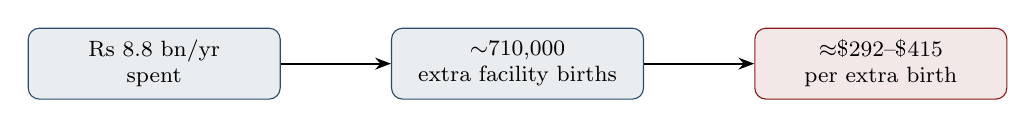
\begin{tikzpicture}[font=\footnotesize, >={Stealth[length=2mm]}, node distance=0.6cm,
      b/.style={draw, rounded corners, fill=jsyblue!10, draw=jsyblue, minimum height=0.9cm, align=center, minimum width=3.2cm}]
    \node[b] (spend) {Rs 8.8 bn/yr\\spent};
    \node[b, right=1.4cm of spend] (extra) {$\sim$710{,}000\\extra facility births};
    \node[b, right=1.4cm of extra, fill=jsyred!10, draw=jsyred] (cost) {$\approx$\$292--\$415\\per extra birth};
    \draw[->,thick] (spend) -- (extra);
    \draw[->,thick] (extra) -- (cost);
  \end{tikzpicture}
  \end{center}
  \vspace{0.4em}
  \begin{columns}[T]
    \column{0.5\textwidth}
    \begin{alertblock}{\footnotesize Caveat 1}
      {\footnotesize The cash goes to \textbf{all} facility mothers, including those who would have used a facility anyway. So the marginal cost is understated.}
    \end{alertblock}
    \column{0.5\textwidth}
    \begin{alertblock}{\footnotesize Caveat 2}
      {\footnotesize The spending bought facility \emph{attendance}, not the \emph{survival} that was its goal.}
    \end{alertblock}
  \end{columns}
\end{frame}

% ===============================================================
\begin{frame}{\phantom{Poll}}
  \pollbanner{select all you expect}
  \vspace{0.5em}
  \begin{center}\large\textbf{A per-birth cash payment can have effects\\nobody targeted. Which did the paper find?}\end{center}
  \vspace{0.8em}
  \begin{columns}\column{0.12\textwidth}\column{0.76\textwidth}
    \opt{A}{Women switch from private to public facilities}
    \opt{B}{A small rise in the number of pregnancies}
    \opt{C}{Earlier breastfeeding after birth}
    \opt{D}{More caesarean sections (more medical intervention)}
  \column{0.12\textwidth}\end{columns}
\end{frame}

% ===============================================================
\begin{frame}{Unintended consequences (\S5.3, Table 5)}
  \begin{columns}[c]
    \column{0.60\textwidth}
    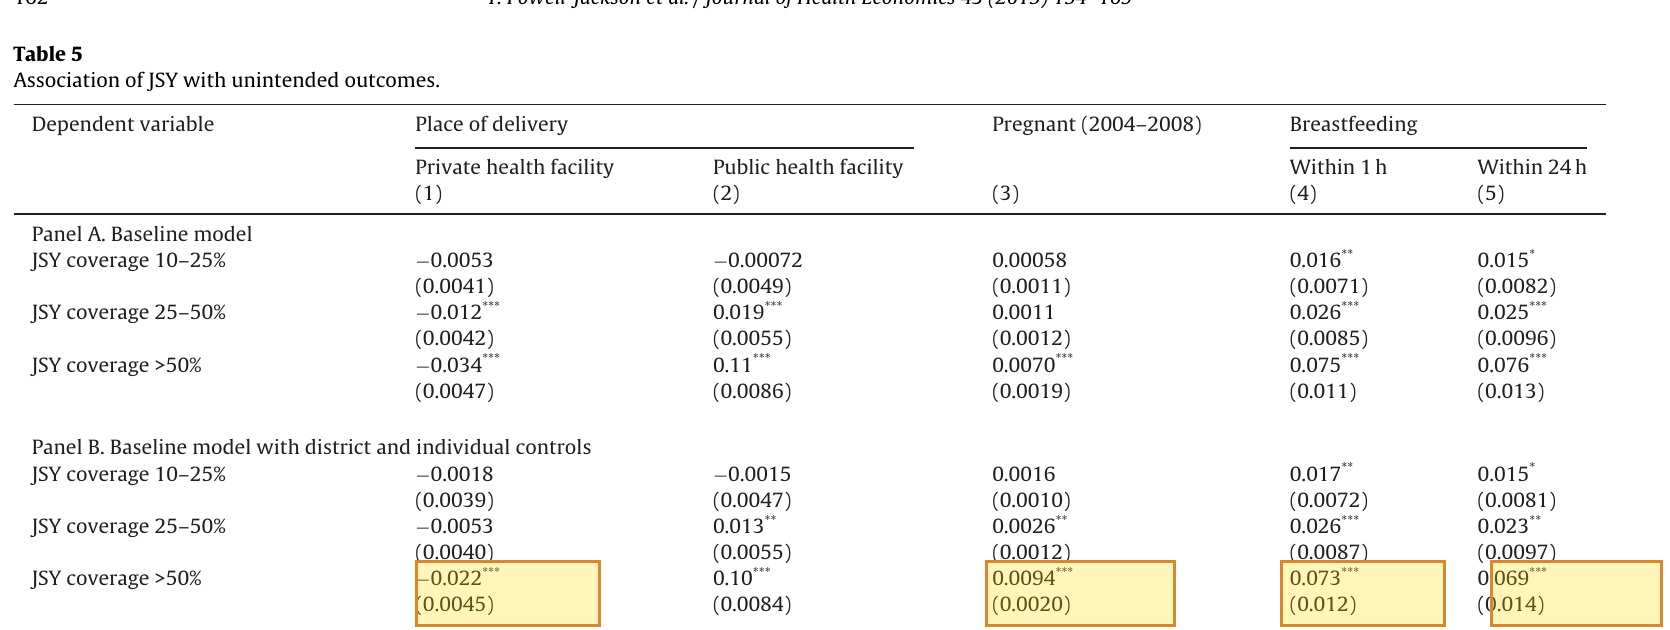
\includegraphics[width=\textwidth]{crop_t5_hl.png}
    \column{0.38\textwidth}
    {\footnotesize \colorbox{jsyamber!30}{Boxed} = the significant $>$50\% effects (Panel B):}
    \begin{itemize}
      \item \textbf{Substitution} (private \kn{$-2.2$ pp}): some new public births are switchers
      \item \textbf{Fertility} (pregnant \kn{$+0.9$ pp}): payment per birth can raise births
      \item \textbf{Information} (breastfeeding \kn{$+7.3$ pp} within 1h, \kn{$+6.9$ pp} within 24h)
    \end{itemize}
  \end{columns}
  \vspace{0.1em}
  \footnotesize Public facility ($+10$ pp) is left unboxed: it restates the main result from Table 3.
\end{frame}

% ===============================================================
\begin{frame}{The fertility result, in the paper's terms}
  \begin{columns}[T]
    \column{0.54\textwidth}
    \textbf{What the authors say.} The JSY rewards a birth, so it may raise fertility, through a shorter birth interval or more children over a lifetime. This can work against the mortality goal (\S2.2, \S5.3).
    \vspace{0.3em}

    \textbf{The design safeguard.} A two-child condition on the cash applied \textbf{only in low-focus states} and was \emph{``difficult to implement''}. DLHS-3 data show the cash reached all parity groups equally (fn. 24).
    \column{0.42\textwidth}
    \begin{alertblock}{The authors' own caveat (fn. 23)}
      {\footnotesize For a woman pregnant at interview, the survey has no start date. The authors \textbf{assign} the pregnancy a random month (3--9) and one of two years.}
    \end{alertblock}
  \end{columns}
\end{frame}

% ===============================================================
\section{Heterogeneity \& robustness (\S6, \S5.4)}
% ===============================================================
\begin{frame}{Heterogeneity by person (\S6, Table 6)}
  \begin{center}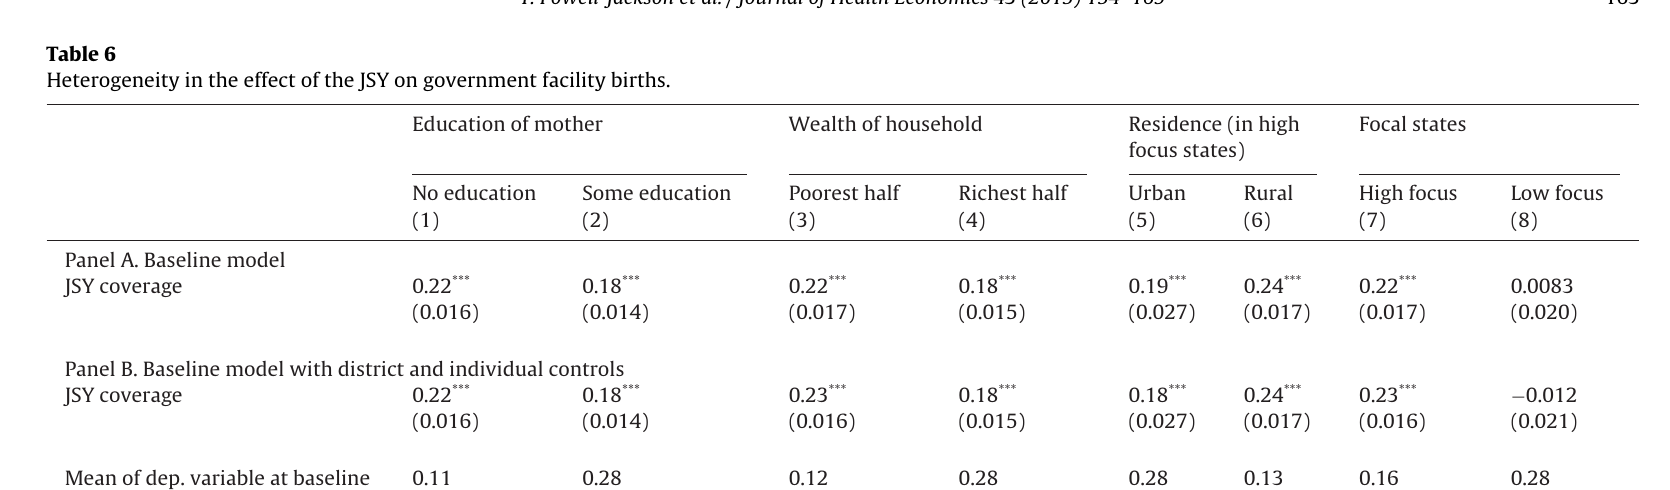
\includegraphics[width=0.96\textwidth]{crop_t6.png}\end{center}
  \vspace{0.2em}
  The authors report that the effect on facility use is:
  \begin{itemize}
    \item \textbf{larger for women with no education} than for women with some education (cols 1--2; $p<0.001$)
    \item \textbf{larger for poorer women} than for richer women (cols 3--4)
  \end{itemize}
  \footnotesize They state that the differences between the subgroups are large relative to the baseline mean.
\end{frame}

% ===============================================================
\begin{frame}{\phantom{Poll}}
  \pollbanner{respond on Slido}
  \vspace{0.5em}
  \begin{center}\large\textbf{The cash is \emph{more generous} in low-focus states.\\Where would you expect the bigger response?}\end{center}
  \vspace{0.8em}
  \begin{columns}\column{0.1\textwidth}\column{0.8\textwidth}
    \opt{A}{Low-focus states --- the bigger cash buys a bigger response}
    \opt{B}{High-focus states --- where the supply system (ASHAs, facilities) was also built up}
    \opt{C}{Whichever started with \emph{lower} facility-birth rates --- more room to grow}
  \column{0.1\textwidth}\end{columns}
  \vspace{0.4em}
  \begin{center}\footnotesize This one is a genuine puzzle --- hold your answer.\end{center}
\end{frame}

% ===============================================================
\begin{frame}{Heterogeneity by amount of cash (\S6, Table 6)}
  \begin{columns}[T]
    \column{0.56\textwidth}
    The authors use the state split to study \textbf{one policy parameter}: how the amount of cash affects the response. The cash is larger in rural areas than urban, and larger in low-focus states than high-focus states.
    \vspace{0.4em}

    They report that the effect was:
    \begin{itemize}
      \item \textbf{larger in rural areas} than urban ($p=0.058$)
      \item \textbf{larger in low-focus states} than high-focus states ($p<0.001$) --- that is, where the cash is more generous
    \end{itemize}
    \column{0.42\textwidth}
    \begin{alertblock}{Read the table with care}
      {\footnotesize The authors' text states the effect is larger in low-focus states. The Table 6 point estimates are high-focus \kn{+0.22} and low-focus \kn{$-0.01$} (n.s.). State the text and the table as the paper reports them.}
    \end{alertblock}
  \end{columns}
\end{frame}

% ===============================================================
\begin{frame}{Robustness (\S5.4)}
  \begin{columns}[T]
    \column{0.5\textwidth}
    \begin{block}{The result holds across}
      \begin{itemize}
        \item Three-year long differences
        \item Dropping high-mortality districts
        \item Dropping low-priority states
        \item Binary and continuous coverage
        \item A pre-trend test that is not rejected
      \end{itemize}
    \end{block}
    \column{0.47\textwidth}
    \begin{alertblock}{State-specific time trends (Panel D)}
      {\footnotesize The authors state this \emph{``reduces the magnitude of the estimates although the general pattern of results remains unchanged''}. The $>$50\% effect falls from \kn{10 pp to 3 pp}.}
    \end{alertblock}
  \end{columns}
\end{frame}

% ===============================================================
\section{Links to the course}
% ===============================================================
\begin{frame}{Back to the opening theme}
  We opened with the \textbf{Ujjwala (LPG)} case: access rose, but the outcome did not follow. The JSY results fit the same pattern.
  \vspace{0.4em}
  \begin{center}
  \begin{tabular}{lll}
    \toprule
    & \textbf{Ujjwala (Gupta et al.)} & \textbf{JSY (this paper)} \\
    \midrule
    Input that rose & LPG ownership ($\approx$75\%) & Facility births ($+8$ pp) \\
    Intended outcome & Clean-air use & Newborn survival \\
    Did it follow? & \textcolor{jsyred}{\textbf{No}} --- solid fuel persists & \textcolor{jsyred}{\textbf{No}} --- mortality flat \\
    \bottomrule
  \end{tabular}
  \end{center}
  \vspace{0.4em}
  \footnotesize The next two slides ask \emph{why} the JSY outcome did not follow, using other course readings.
\end{frame}

% ===============================================================
\begin{frame}{Link: why the supply side matters (Week 3)}
  \begin{columns}[T]
    \column{0.54\textwidth}
    The JSY result turns on the \textbf{quality of public care}. Our Week 3 readings document exactly that problem:
    \vspace{0.3em}
    \begin{itemize}
      \item \textbf{Banerjee, Deaton \& Duflo (2004)}, rural Rajasthan: public staff are often \textbf{absent}, and people bypass public facilities
      \item \textbf{Das \& Hammer (2014)}: low-income settings show a large \textbf{``know--do'' gap} --- providers know more than they do in practice
      \item \textbf{Das et al. (2020), ``Two Indias''}: primary-care \textbf{quality is low}, especially in the public sector
    \end{itemize}
    \column{0.42\textwidth}
    \begin{block}{The connection}
      {\footnotesize These papers give the \textbf{mechanism} the JSY study asserts but does not measure: the facilities women were paid to use may not deliver life-saving care. The supply-side constraint is the course's recurring theme.}
    \end{block}
  \end{columns}
\end{frame}

% ===============================================================
\begin{frame}{Link: incentives and the fertility channel}
  \begin{columns}[T]
    \column{0.5\textwidth}
    \begin{block}{Demand-side incentives (Week 2)}
      {\footnotesize \textbf{Dupas (2011)}, ``Health Behaviour in Developing Countries'', reviews how prices and subsidies shape health demand. The JSY is a textbook demand-side price change, and fits the finding that demand responds but \textbf{health gains are not guaranteed}.}
    \end{block}
    \column{0.5\textwidth}
    \begin{block}{Fertility as a response (Weeks 4, 6)}
      {\footnotesize The JSY's \textbf{fertility side effect} connects to the fertility unit: \textbf{Dehejia \& Lleras-Muney (2004)} on economic conditions and births, and \textbf{Anukriti et al.} on the quantity--quality trade-off. A per-birth payment is an economic shock to fertility.}
    \end{block}
  \end{columns}
  \vspace{0.3em}
  \footnotesize A further contrast: \textbf{RSBY} health insurance (Karan et al. 2017; Prinja et al. 2019, Week 10) is another large Indian demand-side scheme with weak effects on the intended outcome.
\end{frame}

% ===============================================================
\section{Conclusion (\S7)}
% ===============================================================
\begin{frame}{All results on one map}
  \vspace{0.2em}
  \begin{center}
  \resizebox{0.90\textwidth}{!}{%
  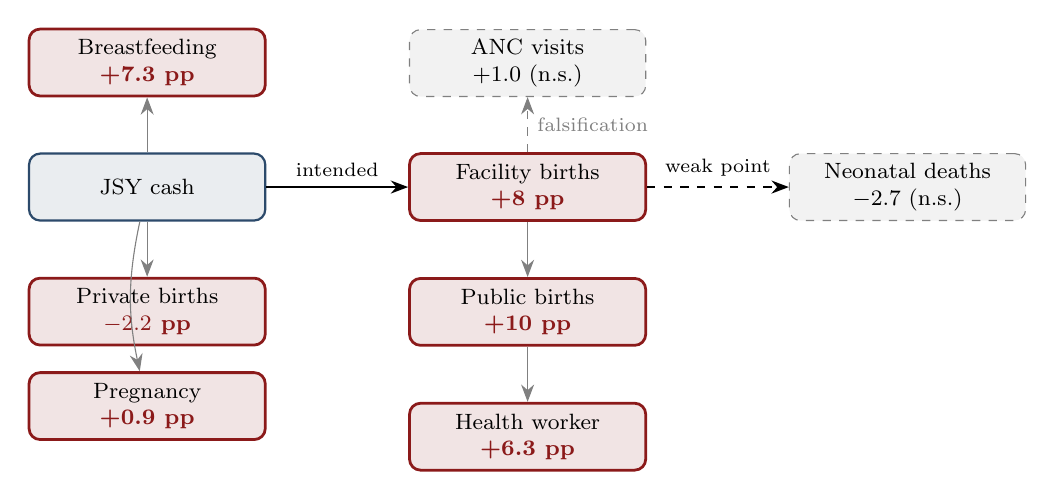
\begin{tikzpicture}[font=\footnotesize, >={Stealth[length=2.2mm]},
      node/.style={draw, rounded corners, minimum height=0.85cm, minimum width=3.0cm, align=center},
      sig/.style={fill=jsyred!12, draw=jsyred, line width=1pt},
      ns/.style={fill=gray!10, draw=gray, dashed},
      core/.style={fill=jsyblue!10, draw=jsyblue, line width=0.8pt}]
    \node[node, core] (cash) {JSY cash};
    \node[node, sig, right=1.8cm of cash] (fac) {Facility births\\\kn{+8 pp}};
    \node[node, ns, right=1.8cm of fac] (mort) {Neonatal deaths\\$-2.7$ (n.s.)};
    \draw[->, thick] (cash) -- node[above,font=\scriptsize]{intended} (fac);
    \draw[->, thick, dashed] (fac) -- node[above,font=\scriptsize]{weak point} (mort);
    \node[node, sig, below=0.7cm of fac] (pub) {Public births\\\kn{+10 pp}};
    \node[node, sig, below=0.7cm of pub] (hw) {Health worker\\\kn{+6.3 pp}};
    \draw[->, gray] (fac) -- (pub); \draw[->, gray] (pub) -- (hw);
    \node[node, ns, above=0.7cm of fac] (anc) {ANC visits\\$+1.0$ (n.s.)};
    \draw[->, gray, dashed] (fac) -- node[right,font=\scriptsize]{falsification} (anc);
    \node[node, sig, above=0.7cm of cash] (bf) {Breastfeeding\\\kn{+7.3 pp}};
    \node[node, sig, below=0.7cm of cash] (sub) {Private births\\\kn{$-2.2$ pp}};
    \node[node, sig, below=1.9cm of cash] (preg) {Pregnancy\\\kn{+0.9 pp}};
    \draw[->, gray] (cash) -- (bf);
    \draw[->, gray] (cash) -- (sub);
    \draw[->, gray] (cash) to[bend right=12] (preg);
  \end{tikzpicture}}
  \end{center}
  \vspace{0.2em}
  \begin{center}{\small \textcolor{jsyred}{\textbf{Red}} = significant, \textcolor{gray}{grey dashed} = not significant. A summary of the results in Tables 3, 4 and 5.}\end{center}
\end{frame}

% ===============================================================
\begin{frame}{Limitations stated by the authors}
  The authors state these limitations in the paper.
  \begin{itemize}
    \item \textbf{Endogeneity.} The authors write that they \emph{``cannot rule out''} confounding. Districts may have adopted the JSY early because of other changes (\S1, \S4)
    \item \textbf{The assumption cannot be tested.} It is \emph{``by definition impossible to test''} the parallel-trends assumption formally (\S5.4)
    \item \textbf{The treatment measure.} JSY coverage is \emph{``mechanically linked to the fraction of women giving birth in a facility''}, so it is an imperfect measure of treatment (\S2.3)
    \item \textbf{Imprecise mortality estimate.} The confidence intervals are \emph{``not sufficiently tight to reject modest effects''} on mortality (\S5.1, \S7)
    \item \textbf{The pregnancy measure.} For a woman pregnant at interview, the authors \textbf{impute} the date of the pregnancy (fn. 23)
    \item \textbf{External validity.} Extending the estimates past 2008 \emph{``may not provide a good approximation to the true impact''} (\S7)
  \end{itemize}
\end{frame}

% ===============================================================
\begin{frame}{Future research, as the authors propose it (\S7)}
  In the conclusion, the authors give these directions for future work.
  \vspace{0.3em}
  \begin{itemize}
    \item Study the \textbf{long-term effects} of financial-incentive programmes, not only the short-term effects
    \item Study the \textbf{potential harms} that such programmes can cause (Lagarde et al., 2007)
  \end{itemize}
  \vspace{0.6em}
  \begin{block}{The authors' main policy point}
    {\footnotesize The evidence on intended and unintended effects points to the need for \textbf{caution} in the use of financial incentives. The supply side must be in place for a demand-side incentive to work, but many schemes run where the quality and availability of care are inadequate.}
  \end{block}
\end{frame}

% ===============================================================
\begin{frame}{The authors' conclusions (\S7)}
  In their own words, the authors conclude:
  \begin{enumerate}
    \item The JSY is associated with an increase in the use of formal health care, \textbf{particularly at lower levels} of the public health system. The increase was \textbf{modest}
    \item The findings on neonatal mortality show \textbf{no strong evidence of an effect}, though the confidence intervals cannot reject modest effects
    \item The evidence on intended and unintended effects points to the need for \textbf{caution} in the use of financial incentives
    \item The supply side \textbf{must be in place} for a demand-side incentive to work
  \end{enumerate}
\end{frame}

% ===============================================================
\begin{frame}
  \begin{center}{\Huge Thank you}\\[1em]{\Large Questions?}\end{center}
\end{frame}

% ===============================================================
\appendix
\begin{frame}{Backup: comparison with Lim et al. (2010)}
  \centering
  \begin{tabular}{lcc}
    \toprule Outcome & Lim et al. (2010) & This paper ($>$50\%) \\ \midrule
    Facility births & +44 to 49 pp & +8.2 pp \\
    ANC (3+ visits) & +11 pp & +1.0 pp (n.s.) \\
    Neonatal mortality & $-2$ to $-6$/1000 & $-2.7$/1000 (n.s.) \\
    \bottomrule
  \end{tabular}
  \par\vspace{0.6em}{\footnotesize The Lim et al. mortality effect is significant in only two of three methods.}
\end{frame}

\begin{frame}{Backup: state-specific trends (Table A7)}
  \centering
  \begin{tabular}{lcc}
    \toprule Public facility delivery & Baseline (Table 3) & State trends (A7) \\ \midrule
    Coverage 10--25\% & $-0.2$ pp & $-1.0$ pp$^{**}$ \\
    Coverage 25--50\% & $+1.3$ pp$^{**}$ & $-1.0$ pp$^{**}$ \\
    Coverage $>$50\% & $+10.0$ pp$^{***}$ & $+3.3$ pp$^{***}$ \\
    \bottomrule
  \end{tabular}
\end{frame}

\begin{frame}{Backup: pregnancy measurement}
  \begin{itemize}
    \item DLHS-3 only. The recall is truncated at 1 April 2001 (2004 for DLHS-3)
    \item For a woman pregnant at interview, the start month is random (3 to 9) and the year is one of two
    \item Table 5, col 3 uses woman-years, so the unit differs from the other columns
  \end{itemize}
\end{frame}

\end{document}
